%%%%%%%%%%%%%%%%%%%%%%%%%%%%%%%%%%%%%%%%%%%%%%%%%%%%%%%%%%%%%%%%%%%%%%%%%%%%%%%%
%2345678901234567890123456789012345678901234567890123456789012345678901234567890
%        1         2         3         4         5         6         7         8

%\documentclass[letterpaper, 10 pt, conference]{./ieeeconf}  % Comment this line out if you need a4paper

\documentclass[a4paper, 10pt, conference]{ieeeconf}      % Use this line for a4 paper

\IEEEoverridecommandlockouts                              % This command is only needed if 
                                                          % you want to use the \thanks command

\overrideIEEEmargins                                      % Needed to meet printer requirements.

% See the \addtolength command later in the file to balance the column lengths
% on the last page of the document

% The following packages can be found on http:\\www.ctan.org
\usepackage{graphicx} % for pdf, bitmapped graphics files
\usepackage[usenames,dvipsnames,svgnames,table]{xcolor}
%\usepackge{amsmat}
%\usepackage{epsfig} % for postscript graphics files
%\usepackage{mathptmx} % assumes new font selection scheme installed
%\usepackage{times} % assumes new font selection scheme installed
\usepackage{amsmath} % assumes amsmath package installed
\usepackage{amssymb}  % assumes amsmath package installed
\usepackage{subcaption}


\newcommand{\paolo}[1]{{\textcolor{red}{#1}}}



\title{\LARGE \bf
Autonomous natural landmarks identification for outdoor navigation
}


\author{
Caterina Massidda$^{*}$,
Heinrich H. B{\"u}lthoff$^{*\dag}$
and Paolo Stegagno$^{*}$% <-this % stops a space
\thanks{$^{*}$C. Massidda, H. H. B{\"u}lthoff and P. Stegagno are with the Max Planck Institute for biological Cybernetics, T{\"u}bingen, Germany. E-mail: \{caterina.massidda, hhb, paolo.stegagno\}@tuebingen.mpg.de.}% <-this % stops a space
\thanks{$^{\dag}$H. H. B{\"u}lthoff is also with the Department of Brain and Cognitive Engineering, Korea University, Seoul, 136-713 Korea.}%
}


\begin{document}


\maketitle
\thispagestyle{empty}
\pagestyle{empty}


%%%%%%%%%%%%%%%%%%%%%%%%%%%%%%%%%%%%%%%%%%%%%%%%%%%%%%%%%%%%%%%%%%%%%%%%%%%%%%%%
\begin{abstract}
Identification of landmarks for outdoor navigation is often performed using computationally expensive computer vision methods or via heavy and expensive multi-spectral and range sensors. Both choices are forbidden on Micro Aerial Vehicles (MAV) due to limited payload and computational power. However, an appropriate choice of the hardware sensor equipment allows the employment of mixed multi-spectral analysis and computer vision techniques to identify natural landmarks. In this work, we propose a low-cost low-weight camera array with appropriate optical filters to be exploited both as stereo camera and multi-spectral sensor.
Through stereo vision and the Normalized Difference Vegetation Index (NDVI), we are able to classify the observed materials in the scene among several different classes, identify vegetation and water bodies and provide measurements of their relative bearing and distance from the robot.
A handheld prototype of this camera array is tested in outdoor environment.
\end{abstract}
%%%%%%%%%%%%%%%%%%%%%%%%%%%%%%%%%%%%%%%%%%%%%%%%%%%%%%Proceedings of%%%%%%%%%%%%%%%%%%%%%%%%%%


%%%%%%%%%%%%%%%%%%%%%%%%%%%%%%%%%%%%%%%%%%%%%%%%%%%%%%%%%%%%%%%%%%%%%%%%%%%%%%%%
\section{INTRODUCTION}\label{sec:introduction}

Recent advances in robotics have made possible a growing number of  real world applications of robotics systems in structured environments, in which external sensors (e.g.: motion capture devices) or artificial {\it a priori} known landmarks are available.
However, in order to employ robotic systems in unstructured outdoor environments, the robots should be able to autonomously identify and select natural landmarks as for example trees and water bodies and collect some relative measurement as bearing and distance.
Among other tasks, this knowledge can be used to achieve localization, plan the action or perform visual servoing.

In most previous works, the identification of particular features in the environment as roads and trees is performed using computationally expensive computer vision algorithms, either employing only cameras or in combination with some range sensor.
In one of the first papers on this topic \cite{94_MaOhYu} the authors fuse the information gathered from a sonar and a camera to measure the relative position of a tree.
However, their method requires many assumptions on the shape of the trees and is suitable only in particular situations.
In \cite{2003_CeDeMH} the authors employ color segmentation in order to extract roads from an image.
In \cite{2008_ZhXiXi}, trees are identified using edge extraction and circular features identification.
Many works \cite{Murrieta-cid02visualnavigation}, 
\cite{2004_ToTo}, \cite{2007_CeAlJi}
 focus on the identification of most salient regions of an image in order to select landmarks for autonomous navigation, independently from the actual type of identified landmark.
%
%
%\medskip
%\cite{2007_CeAlJi} WHAT : natural landmark detection and identification. The former of these previous works builds an environmental model incrementally by using color and stereo range information, while the latter uses a multi-resolution visual attention mechanism to extract image regions most salient in terms of color contrast.
%  Visually-guided navigation system in which a user controls the robot by signaling the navigation target in the images received from a camera transported by the robot.
%SENSOR : camera
%ALGORITHM : Saliency Detection Algorithm.
%APPLICATION : landmark detection, characterization and posterior identification, able to automatically select and track natural landmarks In arbitrary, non-structured environments
%
%\medskip
%\cite{2008_AlGeHe} WHAT /APPLICATION : classification based tree detection method for autonomous navigation of forest vehicles in forest environment. computer vision system that detects tree obstacles on the left and the right side of an autonomous forest vehicle and estimates the distance between a forest vehicle and the base of detected trees in order to make the navigation safe.
%ALGORITHM  : Tree Detection and Distance Measurement (TD\&DM) algorithm has three main parts: Training, Classification, and Segmentation and Distance Measurement.
%SENSOR : camera
%
%\medskip
%\cite{2011_YaRa} WHAT /APPLICATION :  simple contrast-based method for tree detection and shape estimation from ground-plane perspective images for purposes of counting, classification, modeling, or robotic obstacle avoidance. Estimate the position and the size of trees in the scene.
%SENSOR : omnidirectional camera. 
%ALGOROTHM: bar filters as contrast templates to extract vertical features of varying widths in the scene.
%
%\cite{2012_SoSuIa} WHAT : systematical method for extracting tree trunks landmarks from 3D \paolo{point clouds} of cluttered forested environments. 
%ALGORITHM : steps. First, the raw point clouds are segmented by utilizing the circular shape of trees, and segments are grouped into tree sections based on the principle of spatial proximity. Second, circles and axis are extracted from tree sections which are subject to loss of shape information. Third, by clustering and integrating the tree sections resulted from various space inconsistencies, straight tree trunks landmarks are finally formed for future localization.
%SENSOR  : 3D scans of the forested scenes.
%
In \cite{2008_AlGeHe}, a classification approach has been implemented in order to extract tree trunks from the camera images.
The authors of \cite{2011_YaRa} have employed a contrast-based and shape estimation method to estimate the position and the size of trees in the scene through the images gathered by an omnidirectional camera.
With the advent of 3D scanners and RGB-D sensors, similar algorithms (shape identification, clustering) have been applied \cite{2012_SoSuIa} on 3D point clouds.

The problem of the identification of vegetation, water bodies and other materials from satellite and airborn images is well known in remote sensing.
However, it is usually solved exploiting a completely different approach based on the measurement of the reflectance of the Electro-Magnetic (EM) radiation at different wavelengths.
This is done collecting multiple images of the same scene at different wavelengths, not only in the visible spectrum but also in the ultra-violet and in the infrared.
In \cite{2007_BrUnBa}, the authors have employed this principle to identify the vegetation for an autonomous navigation system.
In particular, they have used a cold mirror to split the visible and the Near Infrared (NIR) part of the light among two cameras, and the two resulting images are used to compute the pixel-by-pixel Normalized Difference Vegetation Index (NDVI, see Sect. \ref{sec:background}).
However, their setup, described in \cite{2006_Kelly}, includes many additional sensors as sonars and laser scanners and is not suitable for the application on MAVs.


%\paolo{Some viable alternatives are BUILD YOUR OWN cold mirror and camera array}


In this paper, we are interested in this second approach. % for the identification of natural landmarks in the environment. 
Being our reference platform an MAV, we aim at integrating a low-cost low-weight multispectral sensor in a landmark detection system.
Unfortunately, on-the-shelf multi-spectral sensors are still quite expensive and heavy, hence not suitable for our purpose.
In addition, we would also like to obtain metric information (e.g.: distance, size) of the observed objects, but a normal spectral sensor does not provide it.
In a normal setup, as the one proposed in \cite{2007_BrUnBa}, metric information can only be retrieved by means of additional range sensors, but the limited payload of MAVs does not allow this option.
For this reason, we have decided not to rely on the principle of the cold mirror to design our sensor.

Another interesting attempt to build a low-cost spectral camera relies on the idea of creating an array of cameras and doting each of them with a different optical filter \cite{2012_DoMuHa}.
Similarly, the authors of \cite{2007_LRBLM} outfitted a fixed-wing UAV with an array of sensors including a multi-spectral camera.
One issue that must be addressed in this type of sensor arrays is the matching between corresponding points of the images.
In fact, in order to extrapolate useful data, it is necessary to identify all the pixels in the different images that refer to the same physical object.
Unfortunately, this matching is highly dependent from the distance of the observed object.
Hence, without the knowledge of this distance it is not possible to correctly match the pixels in the images collected at different wavelengths.



%\medskip
%\cite{2004_BrThStRa} WHAT: Robust vegetation detector.  
%SENSOR:  two Sony FCB-EX480 color cameras. One camera is used for visible light and one for NIR by removing the NIR-cut filter. The optical axes of both cameras are aligned using a cold mirror as a beamsplitter.
%APPLICATION : mobile robot navigation
%ALGORITHM = ndvi+ thresholding the result.
%
%\medskip
%\cite{2007_BrUnBa} WHAT : Evaluate the effectiveness of using the NDVI to improve autonomous navigation in natural off-road environment
%APPLICATION : Discrimination between obstacles that most be avoided at all cost, and lesser obstacles which the robot can drive over if necessary
%SENSOR : explained in \cite{2006_Kelly}.  laser scanners and cameras provide the input to the perception system, which consists of 3-D points that have been projected into camera images, and tagged with local properties of the image such as color and the NDVI value (Figure 5). The local perception system then discretizes the space surrounding the robot into a 3-D grid of voxels.
%ALGORITHM : ndvi+spatial distribution of local radar point cloud to classify the region into the surface.
%
%\cite{2006_Kelly} setup of \cite{2007_BrUnBa}







%Ideally, in order to have a 
%One important information to achieve a good classification is the material of which they are constituted.
%In particular, for tasks as autonomous navigation, self landing and autonomous selection of landing areas, it is important to classify sensed objects among a number of different classes, as water and snow, vegetation, soil and man-made materials as concrete and asphalt.
%However, the techniques applied in robotics for this type of classifications are usually based on time-consuming and real-time unfeasible computer vision algorithms with extractions of features, lines and patterns.
%
%The same classification problem is well known and studied by environmental engineers, which usually relies on different principles to classify the earth surface on the basis of satellite imagery.
%The paradigm used in remote sensing is based on the physical principle that the percentage of electromagnetic (EM) radiation reflected by a given material (reflectance) varies with respect to the wavelength of the incident radiation.
%The reflectance of a material constitutes a sort of `unique spectral signature', and can be used  to identify the material itself by comparing online collected data with databases of known materials.
%
%The application of this principle in robotics would allow ....
%
%However, on the shelf spectral cameras are usually expensive and and to heavy to be equipped on Micro Aerial Vehicles (MAV).
%Some attempts to overcome those issues has already been done.

%In general, multi-spectral cameras uses selective mirrors or prisms in order to separate the different wavelengths of the light incident on a single lens, ad project each wavelength on a different sensor.
%The outcome is a set of images of the exact same scene at multiple wavelengths.
%For example, the author of \cite{---}, which for the best of our knowledge is the first and only attempt to use spectral analysis principles into a robotic system, relies on cold mirror to separate the visible and infrared wavelengths and extract vegetation in the observed scenes.


In this work, we propose a sensor design to use the same sensor both as stereo camera and multi-spectral camera, so that we can simultaneously solve the problem of the pixel association in the spectral camera and obtain metric information.
We use two cameras as a stereo pair and compute the corresponding disparity and depth maps.
Using this information, we are able to reconstruct the point of view of the other camera(s), and compute the correct matching for each pixel of the image.
The matched images will then be used to classify the observed objects in a given number of different classes, and finally identify landmarks as objects in the environment of a certain type.
The final outcome is a point-cloud of the landmarks that can be then used in the different tasks of outdoor navigation.
For the best of our knowledge, our system is the first to integrate multi-spectral classification and stereo vision in a single low-cost low-weight sensor that is suitable for the application on MAVs.

The rest of the paper is organized as follows, Section~\ref{sec:background} introduces some background on multi-spectral analysis and the NDVI.
Section~\ref{sec:hardware} describes our hardware setup, while Section~\ref{sec:software_setup} describes the software used to make the online unsupervised classification. Sections~\ref{sec:experimental_setup} and \ref{sec:conclusions} present respectively the experimental results and the conclusions where we describe the future applications and improvements.




%\paolo{infrared active beacons}
%
%\medskip
%\cite{2014_KoOs} WHAT :  They analyze overall infrared technology applications for mobile robot
%localization and they offer a novel localization system based on 1) stationary infrared active beacons and 2) rotary infrared light detection and collimation system installed on moving robot
%APPLICATION : The infrared active beacon approach is arguably the most appropriate for agricultural tasks where repeating determined landmarks are not present




%\paolo{\cite{2009_PuSuHa} journal paper about remote sensing}

%%%%%%%%%%%%%%%%%%%%%%%%%%%%%%%%%%%%%%%%%
\section{BACKGROUND ON SPECTRAL ANALYSIS}\label{sec:background}

Multi-spectral analysis is a powerful technique to classify materials currently applied in many fields as topography, geology, archeology, meteorology among others.
It is based on  the physical principle that the percentage of electromagnetic (EM) radiation reflected by a given material (reflectance) varies with respect to the wavelength of the incident radiation.
The reflectance of a material constitutes a sort of `unique spectral signature', and can be used  to identify the material itself by comparing online collected data with databases of known materials.


%\paolo{spectral signatures of water, vegetation, soil, .... multispectral vs hyperspectral}

Some significant examples of spectral signatures are reported in Fig. \ref{fig:Multispectral}.
The knowledge of such spectral signatures is used to identify the type of observed surfaces.
Ideally, measuring the whole spectral signature of a surface and matching it with the spectral signatures of known materials will allow its identification.
However, sensors able to measure enough points to build the whole spectral signature of an object, known as hyper-spectral cameras, are even more expensive and heavy than multi-spectral cameras.
On MAVs, the sole option is to rely only  on few wavelengths 
%The study of the spectral signatures is generally known as multi- or hyper-spectral analysis, depending on the number of wavelength taken into consideration.

%\paolo{NDVI}

When working under this condition, one technique of spectral analysis consists in developing some mathematical combination of the collected values to accentuate the spectral properties of the targeted materials.
Among those indexes, the NDVI  was developed by NASA to identify vegetation and study its status of health.
Let be $RED$ and $NIR$ respectively the spectral values relative to a surface in the red and Near Infra Red (NIR) bands, then the general equation for the NDVI is:  
%
\begin{equation} \label{eq:ndvi}
\rm NDVI=\frac{NIR-RED}{NIR+RED}
\end{equation}
%
in which the difference of the $NIR$ and $RED$ values is normalized by their sum.
The normalization scales the NDVI to the set $[-1,1]$ and reduces the influence of atmospheric absorption and  the artifacts related to sensor noise.

Since the NDVI is largely used, it is possible to retrieve in literature many values of common materials of outdoor environment, e.g. \cite{2008_PocPar}.
A classification largely accepted in the scientific world differentiate the materials in four main macro-areas $\omega_c, \, c=1, \ldots, 4$, for which some examples of spectral signatures are reported in Fig. \ref{fig:Multispectral}.

The first macro-area $\omega_1$ includes a wide variety of healthy vegetation, and account for the strong absorption in the red band due to clorophilla and the equally strong reflection of the NIR EM radiation of the green vegetation.
The two effects result in high values of the NDVI index  ($\rm{NDVI({\omega_1})}>0.6$).
Low and dry vegetation fall in the category $\omega_2$,  in which the two phenomena are less strong, hence the NDVI values  ($0.2<\rm{NDVI(\omega_2)}<0.6$) are still positive but less than the previous category.
Bare soil, as well as concrete and some other man-made materials, have in general a slightly increasing spectral signature (Fig. \ref{fig:Multispectral}), while the spectral signature of asphalt is nearly flat.
The corresponding NDVI values ($ 0<\rm{NDVI(\omega_3)}<0.2$) are still positive but close to zero.
Finally, water in lakes, rivers and seas, as well as snow, have a stronger absorption in the NIR band with respect to the red band, resulting in negative NDVI values ($\rm{NDVI(\omega_4)}<0$).
%
This classification is summarized in the following equation:
%
\begin{eqnarray}  \label{ndvi_values}
      & &\rm{NDVI(\omega_1)}>0.6 \nonumber\\
      & & 0.2<\rm{NDVI(\omega_2)}<0.6 \nonumber\\
      & & 0<\rm{NDVI(\omega_3)}<0.2\\
      & & \rm{NDVI(\omega_4)}<0 \nonumber.
\end{eqnarray}


%A multispectral remote sensors produce images with a few relatively broad wavelength bands, as known,  the information from different wavelengths of light is collected as in a digital camera. Using this type of sensor,  there are two major differences. The first one is that instead of limiting itself to the visible wavelengths (RGB),  using a multispectral sensor is possible to collect, information in the infrared, coming up until the thermal wavelengths. The second major difference is that instead of automatically combining the information from the different wavelengths to form a picture, the information for each specific wavelength is stored in a separate image. This image is commonly called band and it is similar to a black and white digital photography. Combining the different bands is possible to create false color images, i.e. the combination of green-red-infrared, the blue channel is replaced with near infrared. In this case, plants reflect in the near infrared and green, while absorb in the red. Since the plant reflect more in near infrared than in the green, plant-covered land appears deep red. The ground is gray or tan, and clear water is black.
%
%It is possible to use more bands and have more accurate informations, for doing this is needed a hyperspectral sensor. It collects image data simultaneously in many narrow, adjacent wavelength bands. The development of this complex sensor involved the spectroscopy, Using it, it possible to calculate the spectral reflectance or the spectral, it  is the ratio of reflected energy as a function of wavelength, (Fig.~\ref{fig:Multispectral}). Reflectance varies with wavelength for most materials because energy at certain wavelengths is scattered or absorbed to different degrees. For this reason we have chosen to build a multispectral sensor instead a hyperspectral one  to address our research. It is not possible to use  this sensor in a low cost project, as well as we have done our, in fact its principal  limit is due to the high price of construction. it needs a lot of different bands to work properly.
%
%For the reason above mentioned,  to address our work we have chosen to build a multispectral sensor instead a hyperspectral one.
%
%
%In this work, using a multispectral sensor, we have calculated  the Normalized Difference Vegetation Index (NDVI) it is one of the most commonly used vegetation indexes this is due to the ease of calculating it. The NDVI is calculated on a per-pixel basis as the normalized difference between the red and near infrared (NIR) bands from an image. It is an index of plant “greenness” or photosynthetic activity.  As shown in \cite{2008_PocPar} it also possible to use it to discern the limits of four different macro areas: water, soil, tress and grass.  This is possible because they have a different spectral signature, amount of electro-magnetic radiation reflected, as shown in Fig.~\ref{fig:Multispectral}.
%
% Until now the major limitation of use this technique was the cost and weight of this kind of cameras. in fact a low cost multispectral camera is likely very heavy, and a lighter one is very expensive. In several works is shown that is possibly to make a low cost multispectral camera. For example,  in  \cite{2012_DoMuHa} is described a system that uses an array of mobile camera  modules and filters to record images in distinct and arbitrary bands in the ultraviolet (UV) to NIR region of the electromagnetic spectrum.
%
%However, using this type of configuration for the cameras there is the problem, not yet solved,  of associating pixels amongst different cameras, in particular objects at different distances produce different associations of pixels.For this reason, the second task of this work was to find a solution to it. We have managed the problem implementing a disparity map and using it to find the correct associations of pixels.
%
%HOWEVER, THE PROBLEM OF ASSOCIATING PIXELS AMONGS DIFFERENT CAMERAS IS YET NOT SOLVED.
%
%IN PARTICULAR, OBJECTS AT DIFFERENT DISTANCES PRODUCE DIFFERENT PIXEL ASSOCIATIONS.
%
%In this paper we have made a low cost and weight camera, and we had used it for an online unsupervised classification of the video. For the best of our knowledge this work is the first one that combines the study and the solution of  this three points: cost, weight and online unsupervised classification.





\begin{figure}[t]
      \centering
      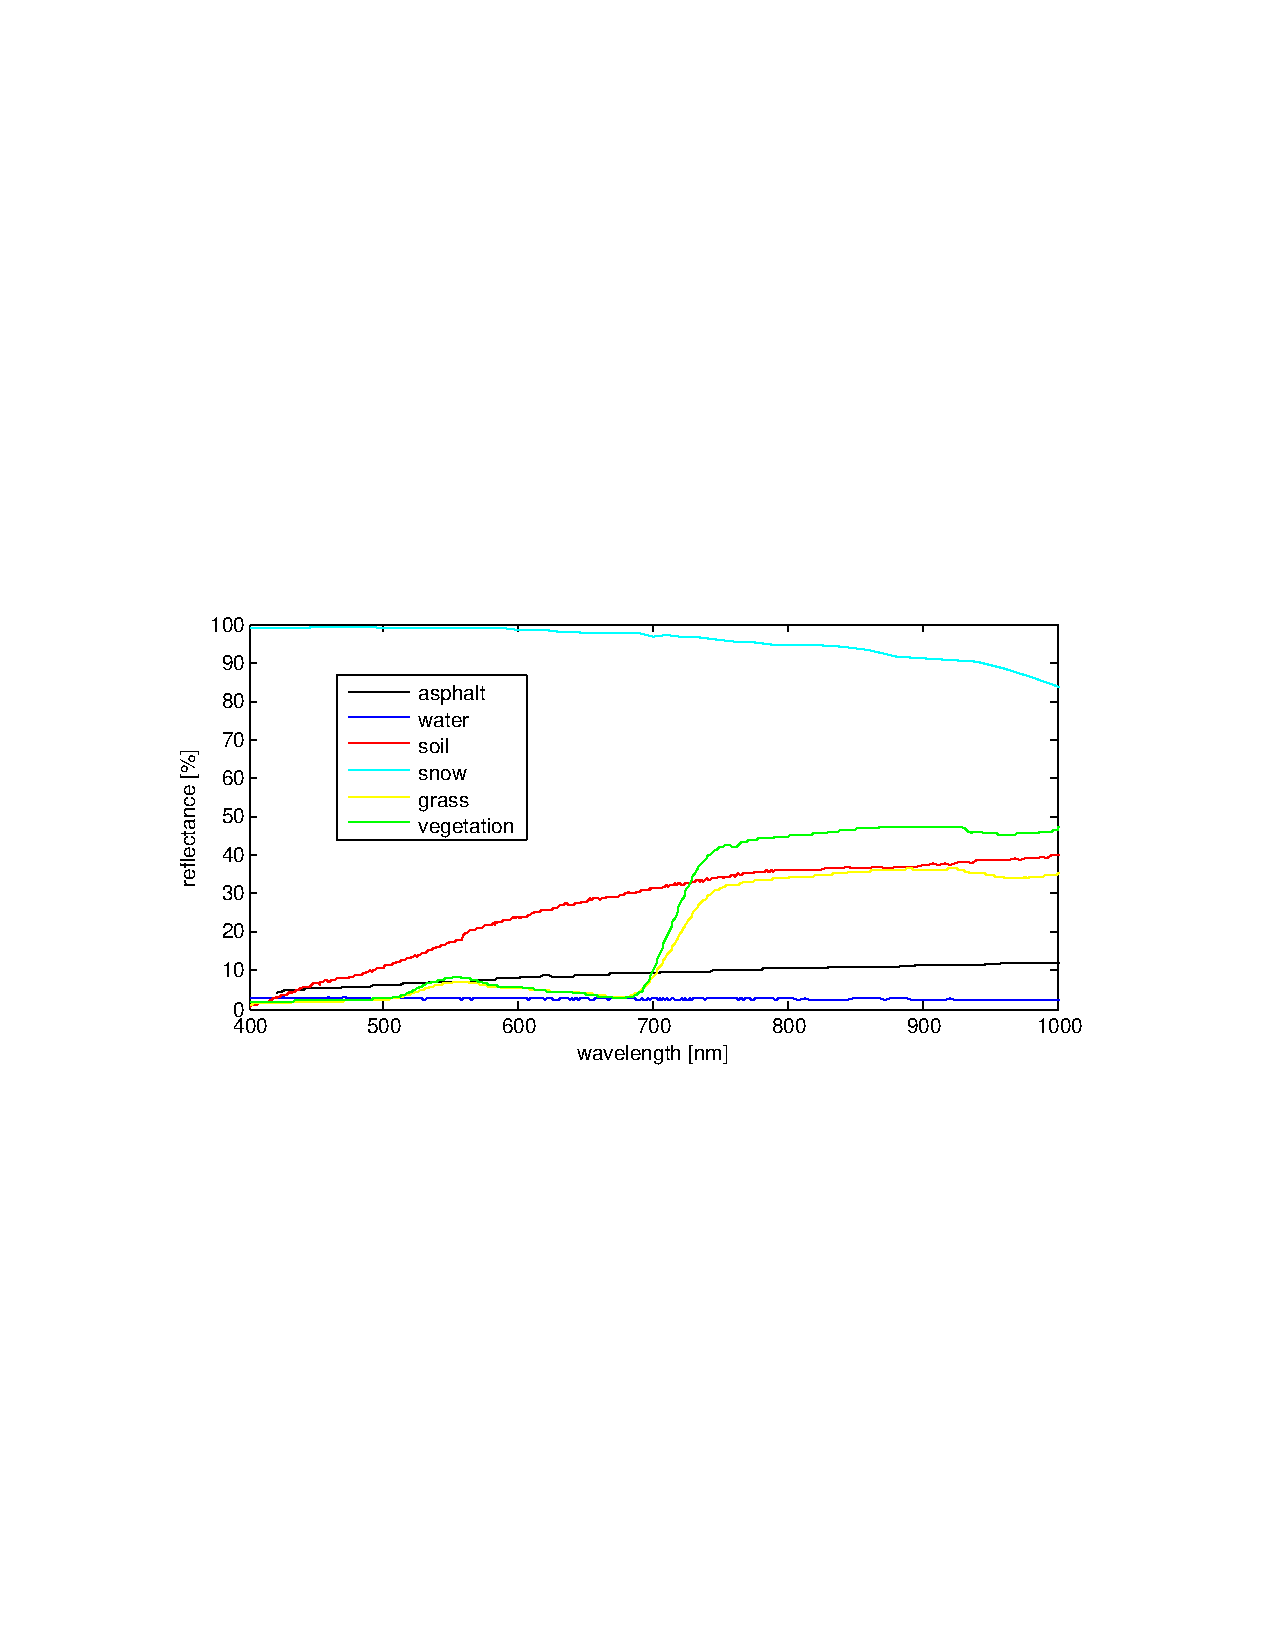
\includegraphics[trim = 12mm 99mm 12mm 99mm, clip,width=0.99\linewidth]{../images/multispectralSignature.pdf}
      \caption{Spectral signatures of some materials \cite{2009_BaHoGrRi}. }
      \label{fig:Multispectral}
   \end{figure}




%%%%%%%%%%%%%%%%%%%%%%%%%%%%%%%%%%%%%%%%%%%%%%%%%%%%%%%%%%%%%%%%%%%%%%%%%%%%%%%%
%\section{SYSTEM OVERVIEW}\label{sec:system_overview}


%The camera array is composed by three cameras mounted in a straight line on a 3D printed frame shown in  Fig.~\ref{fig:Cadmodel}.
%The cameras on the right and left side are equipped with a dark red filter (wavelength = 660 [$ nm $]). In this band the green vegetation appears darker than in the other visible light bands. The strength of this absorption can be used to differentiate different type of plant and to determine soil color. The central camera is equipped with a near infrared filter (wavelength = 850 [$ nm $]). In this band the green vegetation is much brighter than in any visible bands, while the water appears very dark, due to its strong absorption of near infrared radiation.

%Each camera takes a frame in the same instant, collecting three images from three different points of view of the same scene. Using the frames taken by RedL and RedR we are able to compute the disparity map and to reconstruct the point of view of $NIRC$. We refer to the reconstructed image RedL and RedR as $RedC$.
%The following step is to compute value of the NDVI of the environment captured by the cameras
%for each pixel of the central image using the corresponding pixel of $RedC$. Therefore we are able to classify each pixel of the central image in a number of subclasses (e.g.: water, soil, grass, trees). However, the classified image present many outliers and is effected by substantial noise. In order to improve the quality of the NDVI classification we apply a fuzzy clustering algorithm  on the NDVI image.


%%%%%%%%%%%%%%%%%%%%%%%%%%%%%%%%%%%%%%%%%%%%%%%%%%%%%%%%%%%%%%%%%%%%%%%%%%%%%%%%
\section{HARDWARE SETUP}\label{sec:hardware}

The camera array consists of three USB 2.0 mvBlueFOX grayscale cameras mounted in a straight line on a 3D printed frame shown in  Fig.~\ref{fig:Cadmodel}.
The cameras have a resolution of 752x480 pixels and offer a complete control to the user, allowing for example external triggering and the setup of the exposition time.
In the following, we will refer the left, central and right cameras respectively as $CamL$, $CamC$, and $CamR$. 
$CamC$ is positioned in the middle between $CamL$ and $CamR$.

Each camera is equipped with an S-mount low distortion $(dis< 0.2 \% )$ Lensagon B5M41430ND lens.
The $CamL$ and $CamR$ lenses are equipped with a dark red bandpass filter (wavelength = 660 [$ nm $]) with a diameter of $ d=22.5 [mm]$.
The $CamC$ lens is equipped with an infrared bandpass filter (wavelength = 850 [$ nm $]) with the same diameter.
The frame with the cameras, lens and filters  are shown in Fig.~\ref{fig:camera}.
This layout allows us to use the $CamL$ and the $CamR$ as stereo camera.

An important factor in the choice of the camera and the lenses is their efficiency with respect to the different wavelengths.
In particular, we considered the quantum efficiency $QE$ of the camera sensor and the transmission efficiency of the filters.
The two contributions must be considered together in order to obtain the  total efficiency of the filter/camera sensor system.
%
The $QE$ is related to the ability of the sensor to respond to the incoming photon signal and to its conversion into a measurable electron signal.
The $QE$ is usually expressed as the probability that a photoelectron will be released for each incident photon, and is in general a function of the wavelength $\lambda$ of the incident light ($QE\triangleq QE(\lambda)$).
The chosen sensor is sensible in the bands of interest (red and NIR).

The transmission efficiency of the filters is the ratio of the transmitted power over the incident power, and is again a function of the wavelength $\lambda$. In our case, we refer to the transmission efficiency of the red and NIR filters respectively as ${TE}_{Red}$ and  $TE_{NIR}$.
The plots of the total efficiency of the red and NIR filters/camera systems with respect to the wavelength $\lambda$, respectively $E_{Red}(\lambda)=QE\cdot TE_{Red}$ and $E_{NIR}(\lambda)=QE \cdot TE_{NIR}$, are shown in Fig.~\ref{fig:reflectance}, along with $QE$, $TE_{Red}$ and  $TE_{NIR}$.

%The choice of the filter bandwidth was dictated by our final goal for this work.
%In fact, we choose the standard values 
%The cameras on the right and left side are equipped with a dark red filter (wavelength = 660 [$ nm $]). In this band the green vegetation appears darker than in the other visible light bands. The strength of this absorption can be used to differentiate different type of plant and to determine soil color. The central camera is equipped with a near infrared filter (wavelength = 850 [$ nm $]). In this band the green vegetation is much brighter than in any visible bands, while the water appears very dark, due to its strong absorption of near infrared radiation.


The three cameras are connected through USB ports to an i5 PC which runs the software to acquire the camera images and performs the unsupervised classification of the observed objects.
The overall weight of the 3D printed frame, cameras, lenses and filters is $\simeq100g$, while the total cost of those components is below 1000 Euros.

\begin{figure*}[t]
        \centering
\begin{subfigure}[t]{0.45\textwidth}
        \centering
	     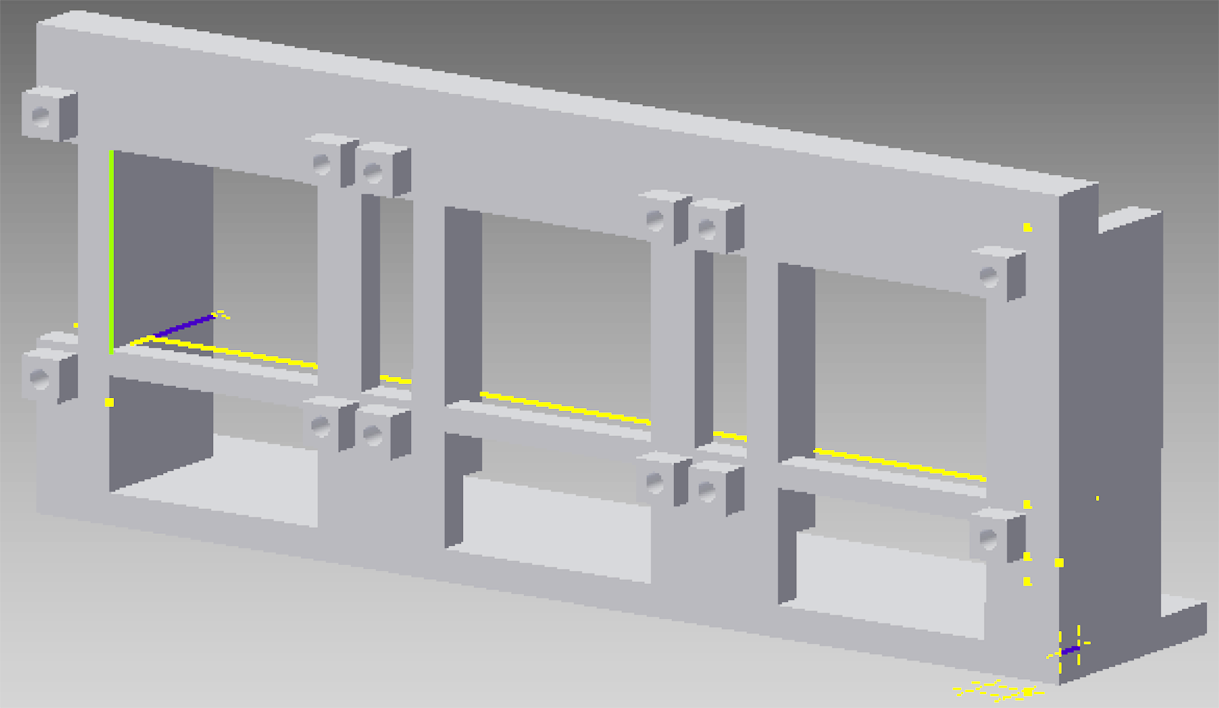
\includegraphics[width=0.9\linewidth]{../images/support_camera_3x1.png}
      	\vspace{-0.2cm}
    		\caption{} 
		\label{fig:Cadmodel}
    \end{subfigure}%
    ~ 
    \begin{subfigure}[t]{0.5\textwidth}
        \centering
      	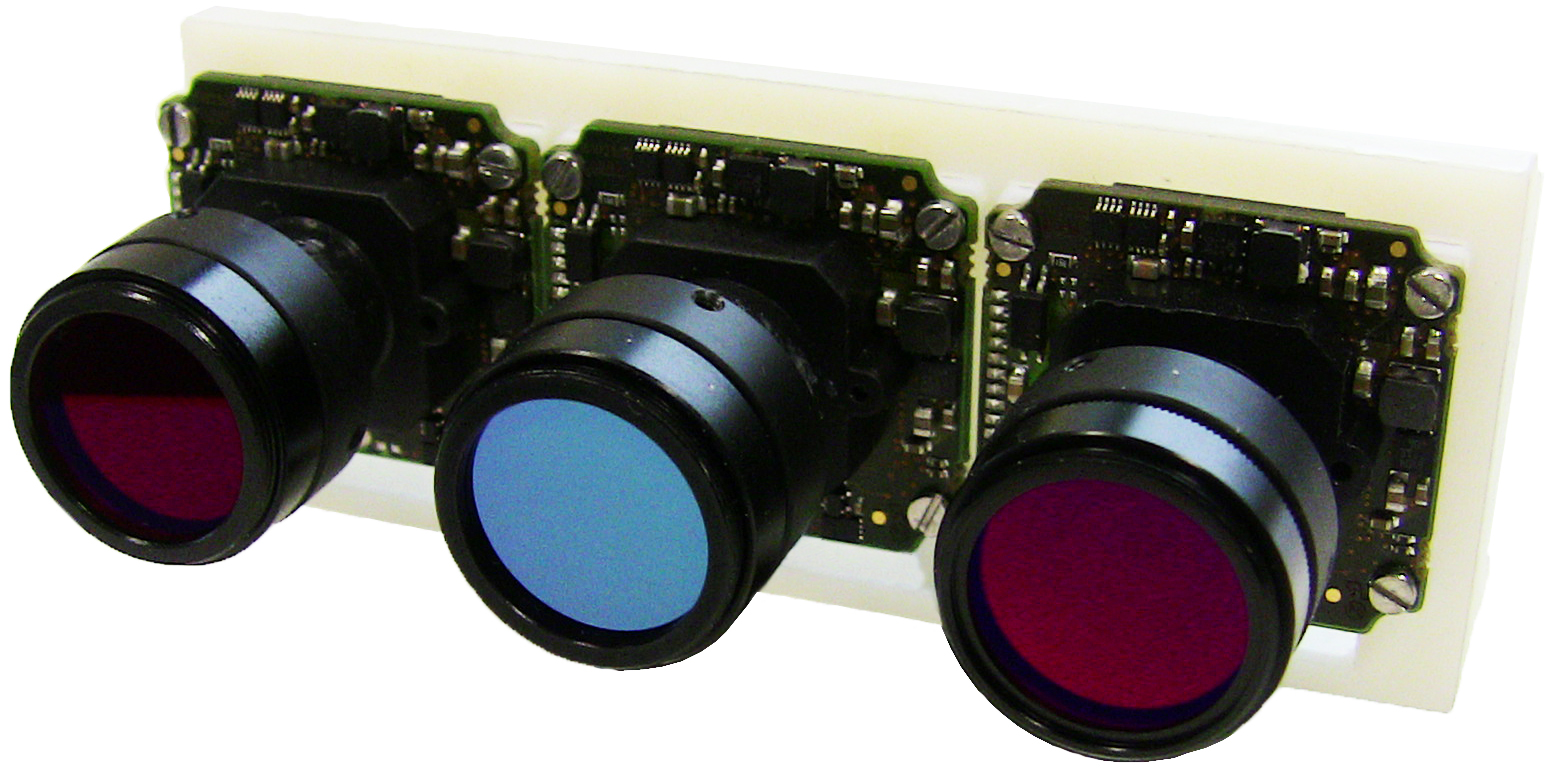
\includegraphics[width=0.9\linewidth]{../images/IMG_0198.JPG}
      	\vspace{-0.2cm}
      	\caption{}
     		\label{fig:camera}
    \end{subfigure}
    \caption{(a) the cad model of the camera support; (b) the camera array with lenses and filters.}
\end{figure*}
   
   
   
   \begin{figure}[t]
      \centering
      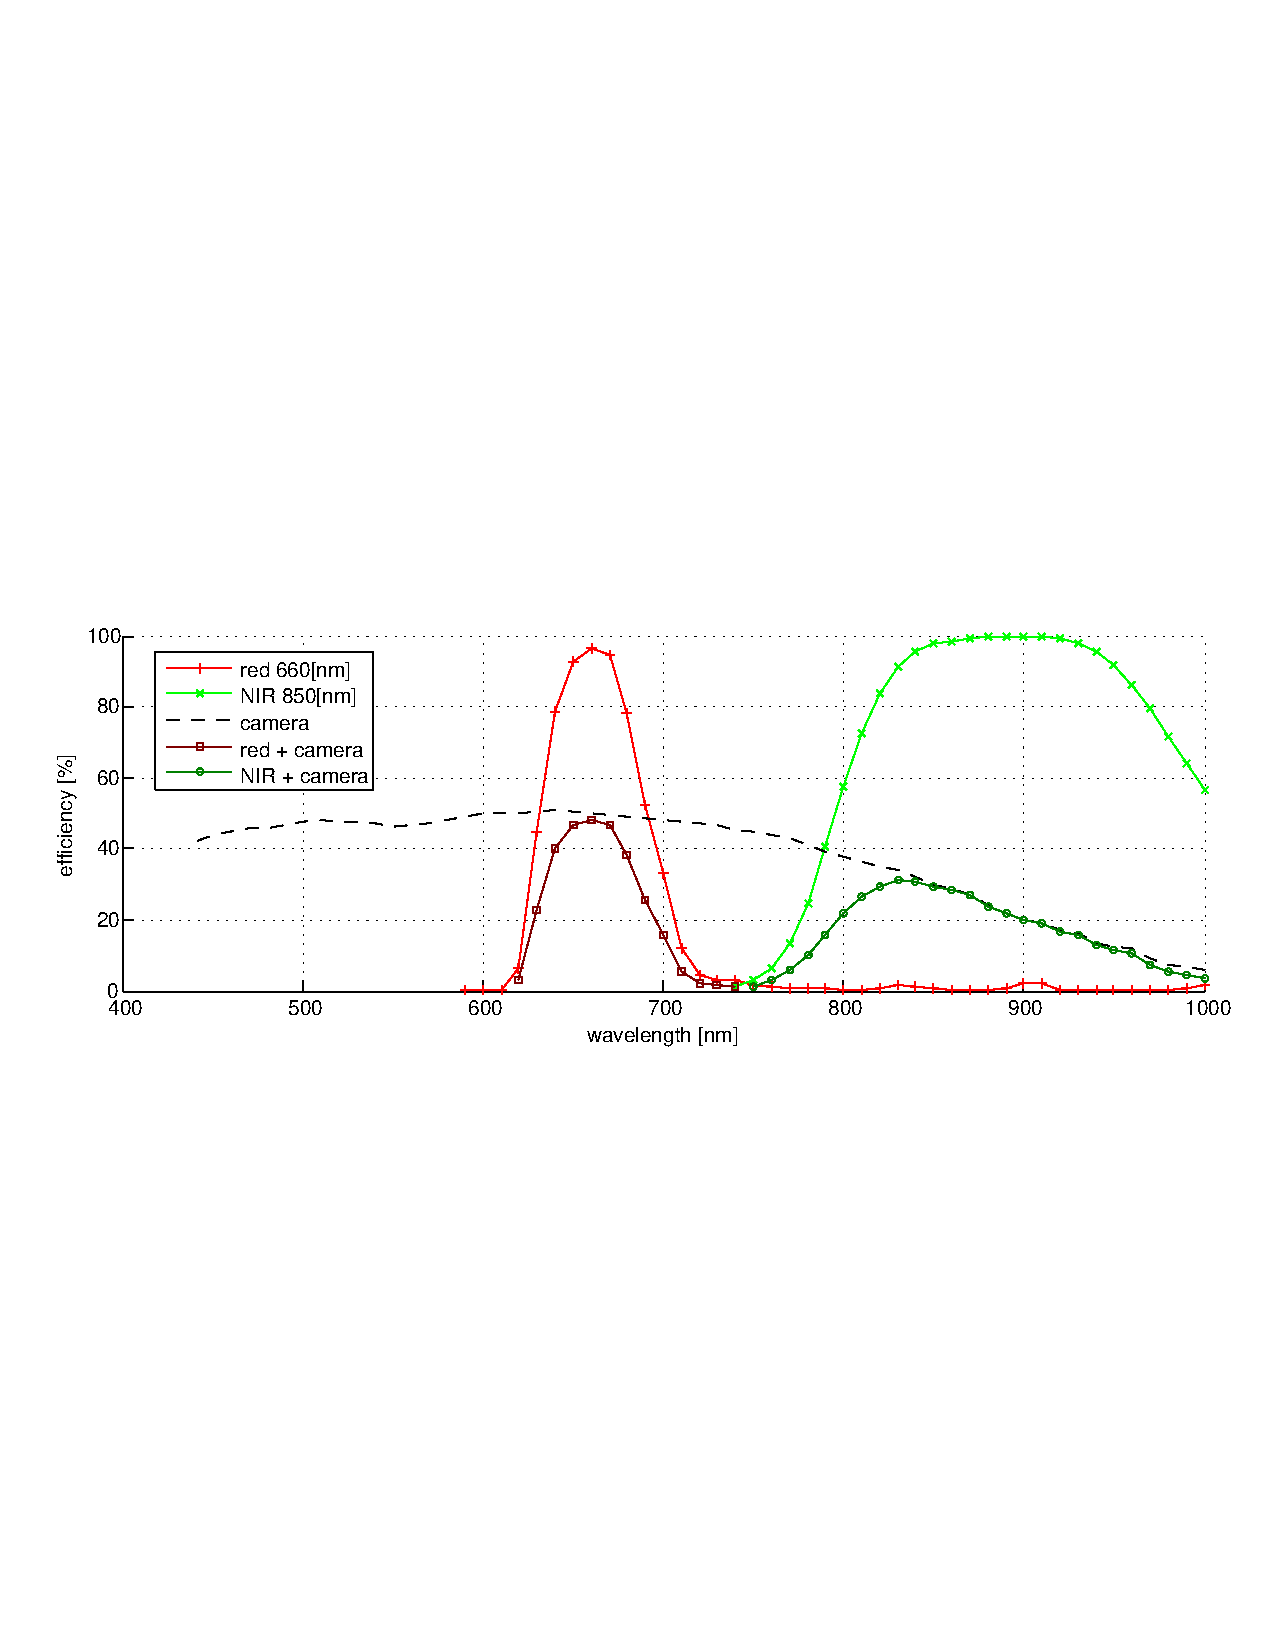
\includegraphics[trim = 10mm 99mm 10mm 99mm, clip,width=0.99\linewidth]{../images/plot_reflectance.pdf}
      \caption{Widths and efficiency of the two filters used in the multispectral sensor. The light red and dark red plots show respectively the transmission efficiency of the red filter and of the red  filter mounted on the camera. The light green and dark green plots show respectively the transmission efficiency of the NIR filter and of the NIR  filter mounted on the camera. The dark dashed line shows the quantum efficiency of the camera sensor.}
     \label{fig:reflectance}
   \end{figure}


%%%%%%%%%%%%%%%%%%%%%%%%%%%%%%%%%%%%%%%%%%%%%%%%%%%%%%%%%%%%%%%%%%%%%%%%%%%%%%%%
\section{SOFTWARE SETUP}\label{sec:software_setup}


The software to acquire the camera images and perform the unsupervised classification encompasses several components.
A block scheme of the whole system is provided in Fig. \ref{fig:Blockdiagram}, and will be the reference for the reader throughout this Section.
In general, we will denote the images gathered from the left, central and right cameras respectively as $RedL$, $NIRC$ and $RedR$.
Each camera captures a frame in the same instant, collecting three images from three different points of view of the same scene.

A precondition to perform the classification is to ensure that the images contains useful information by an appropriate selection of the exposition times of the cameras.
If the exposition of a camera sensor is too long the gathered image will be all white, while a too short exposition will result in a dark image.
Since $CamR$ and $CamL$ will be used as a  stereo pair, it is in general good practice to select the same exposition time $ExT_{Red}$ for both cameras, while the exposition time $ExT_{NIR}$ of $CamC$ can be set independently.
Thereafter, we implemented two independent  PID controllers to regulate the brightness of the images, using as input the mean value of the pixels of the images.

%**** MAYBE PUT EQUATIONS????


Once the images are acquired, they are passed on to the system responsible for the classification.
The first step is to find the correspondences among the pixels of $RedL$ and $RedR$ and the pixels of $NIRC$, or equivalently to reconstruct with $RedL$ and $RedR$ the same point of view of $NIRC$.

As mentioned in Section~\ref{sec:hardware}, this is done by using $CamL$ and $CamR$ as a stereo camera.
The software computes the disparity map $D_{Red}$ of $RedL$ and $RedR$ and uses it to reconstruct the same point of view of the central camera $CamC$.
In this way, we have two images $RedC(RedL, RedR)$ and $NIRC$ taken from the same point of view with two different bands.
From $RedC$ and $NIRC$ it is possible to compute the pixel by pixel NDVI value to obtain the NDVI matrix, denoted by $NDVI$, as we will show in Section~\ref{sec:NDVI}.
This can be used to classify the surfaces according to standard values known from literature.

However, since $NDVI$ is usually corrupted by consistent noise (due to e.g.: mismatches in the association, difference in the illumination, etc.), the classification is conducted considering spatial information in addition to spectral information.
The application of such clusterization algorithm, which we will explain in detail in Section~\ref{sec:clustering} and is based on \cite{1997_Wiemker}, leads to a consistent reduction of outliers and erroneous classifications. 

%The result is obtained has some noise, in fact the four macro-areas are not very well recognizable. To solve this problem, we have applied to the NDVI a fuzzy clusterization using spectral-spatial informations.  Using this mathematical combination, the software is able to subdivide the image in four distinct macro-area (trees, grass, soil and water). It will be able to use this information, for example , to extract features.




\begin{figure}[t]
      \centering
      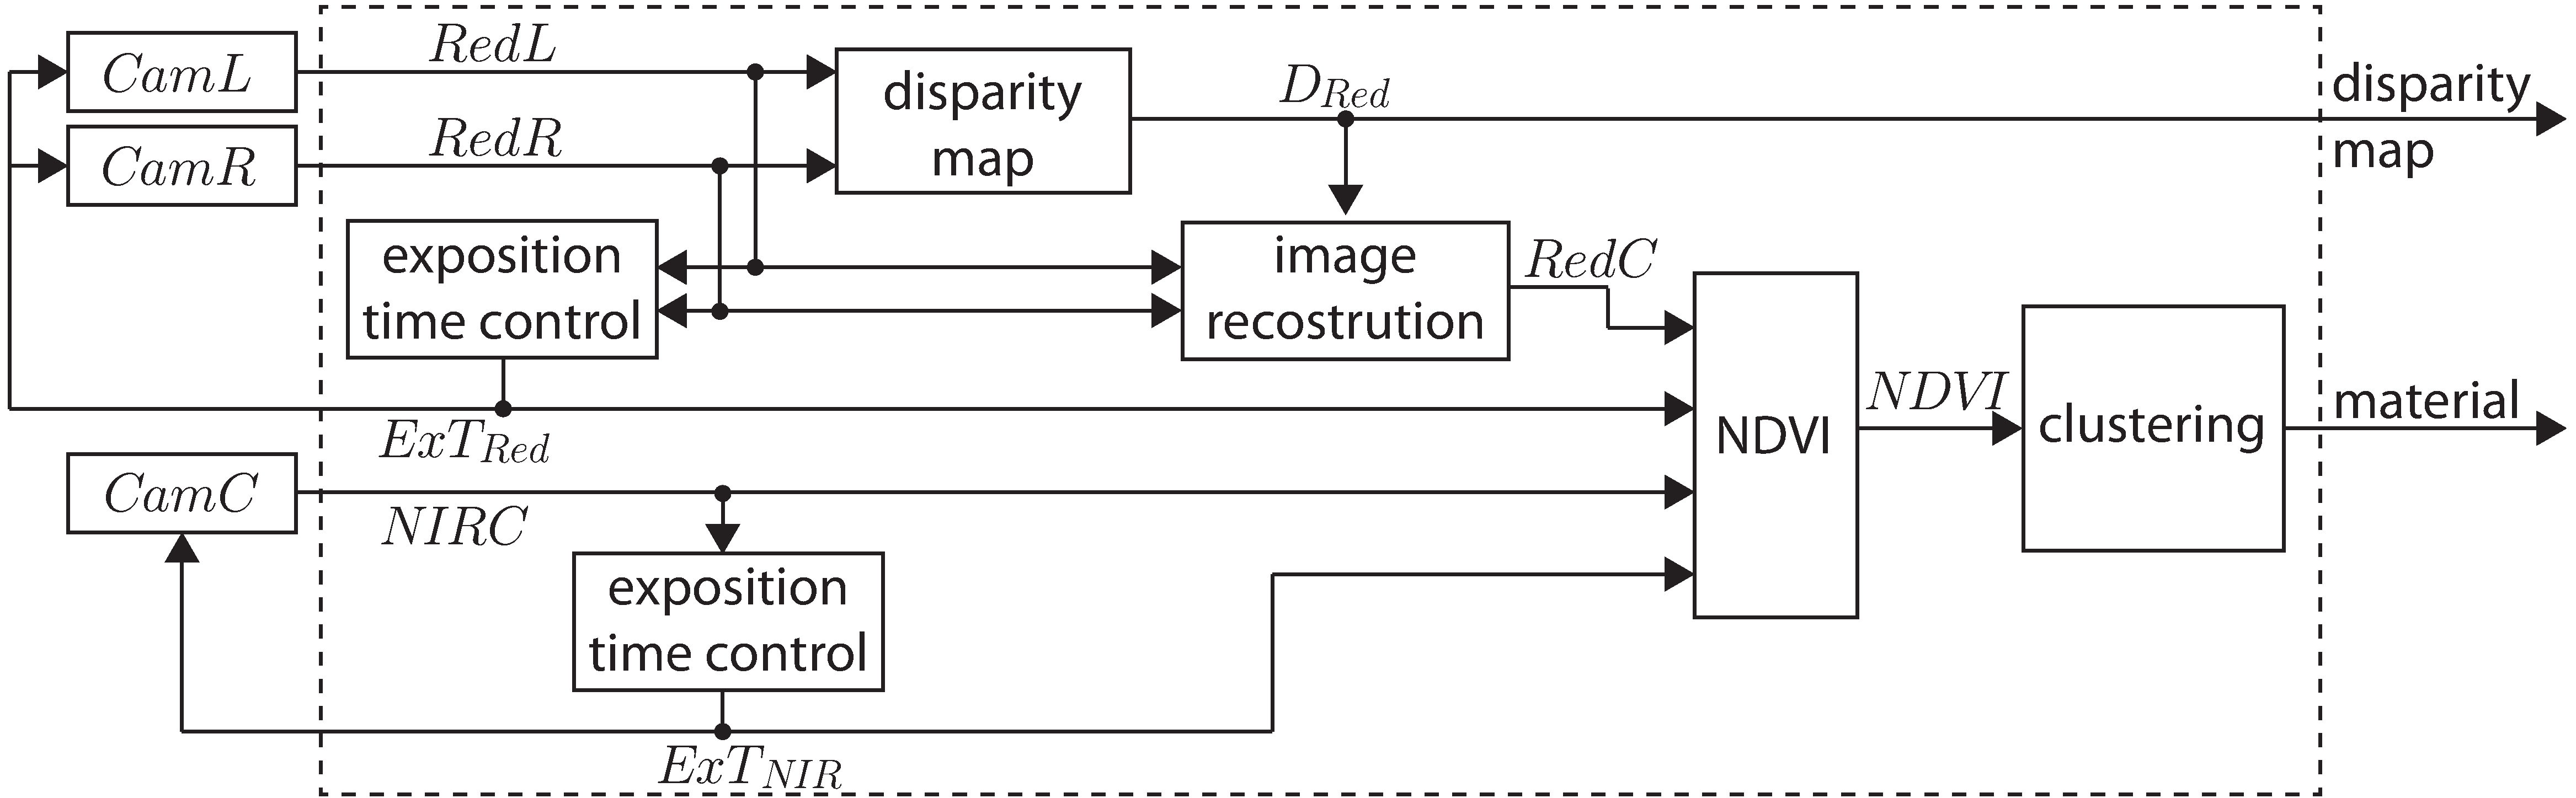
\includegraphics[width=0.99\linewidth]{../images/diagram_ndvi_plus_disparity.pdf}
      \caption{Block diagram of the developed system.}
     \label{fig:Blockdiagram}
   \end{figure}



%In this work, we have made a software to have an unsupervised classification of the video recorded by the multispectral sensor.  uses a pixel based classification and  utilizes the fuzzy clusterization with the spatial information \cite{1997_Wiemker}.






\subsection{NDVI}\label{sec:NDVI}

The matrix $NDVI$ cannot be computed directly on the pixel values of $RedC$ and $NIRC$.
In fact, two more factors must be considered to apply equation \eqref{eq:ndvi}.
First, since the exposition times are set independently as $ExT_{red}$ for $CamR$ and $CamL$,  and as $ExT_{NIR}$ for $CamC$ camera, we need to consider their difference by applying to the values in $RedC$ a multiplicative correction factor $\delta$:
%
\begin{equation} \label{exposition}
\delta=\frac{ExT_{NIR}}{ExT_{red}}\;.
\end{equation}

The second factor is the difference in the efficiency of the filter/camera systems in the two bands.
In particular, the total efficiencies $Tot_{red}$ and $Tot_{NIR}$ of the red filter/camera and NIR filter/camera are respectively:
%
\begin{eqnarray}  \label{integral}
Tot_{red} &=  \int E_{red} d\lambda =303.07\nonumber\\
Tot_{NIR} &=  \int E_{NIR} d\lambda=433.62 \;.
\end{eqnarray}
%
However, equation \eqref{eq:ndvi} requires pure spectral values collected by sensors with the same efficiency in order to be applied.
Hence, another multiplicative correction factor $\alpha$ must be applied to $RedC$:
%
\begin{equation}\label{alfa}
\alpha=\frac{Tot_{red}}{Tot_{NIR}}=1.43 \;.
\end{equation}

Considering the value of a pixel from the reconstructed image ${RedC}_{i,j}$  and the corresponding  pixel in the  ${NIRC}_{i,j}$ and considering the two correction factors (\ref{exposition}) and (\ref{alfa}), the pixel-by-pixel NDVI values must be computed as:
%
\begin{equation} \label{eq:ndvi_new}
NDVI_{i,j}=\frac{NIRC_{i,j}-RedC_{i,j}\cdot \alpha \cdot \delta}{NIRC_{i,j}+RedC_{i,j}\cdot \alpha\cdot \delta}
\end{equation}
where $NDVI_{i,j}$ is the element at the $i$-th row and $j$-th column of the matrix $NDVI$.

%%%%%%%%%%%%%%%%%%%%%%%%%%%%%%%%%
\subsection{Clustering}\label{sec:clustering}
%%%%%%%%%%%%%%%%%%%%%%%%%%%%%%%%%

Using $NDVI$ computed through equation~\eqref{eq:ndvi_new} it is possible to classify the observed materials, i.e.: to assign to each pixel $x_{i,j} \in NDVI$ a label $\omega_{i,j}$ among the set of possible labels $\Omega=\{\rm{\omega_1, \omega_2, \omega_3, \omega_4}\}$ following the rules in equation~\eqref{ndvi_values}.
For visualization purpose, the $\omega_{i,j}$ can be collected in an image $Cl$ whose pixels $Cl_{i,j}$ are defined as a function of $\omega_{i,j}$: $Cl_{i,j}=Cl_{i,j}(\omega_{i,j})$.

However, due to possible mismatches between $RedC$ and $NIRC$, difference in the illuminations, etc., $NDVI$ will be affected by consistent noise and $Cl$ will contain many errors in the classification.
Hence, we apply a more robust classification based on the fuzzy K-means clusterization, whose first step consists in computing for each pixel $x_{i,j} \in NDVI$ the  membership values 
%
\begin{equation}  \label{integral}
P_{spec}(x_{i,j}|\omega_c) =  \frac{\Lambda_c(x_{i,j})}{ 	\sum_{h=1}^4 \Lambda_h(x_{i,j})}, \; c=1, \ldots, 4
\end{equation}
where $\Lambda_c(x_{i,j})$ is the probability that a surface of class $\omega_c$ produces an NDVI value equal to $x_{i,j}$.
Note that $\sum_{c=1}^n P_{spec}(x_{i,j}|\omega_c)=1$, hence $P_{spec}(x_{i,j}|\omega_c), \, c=1, \ldots, 4$ is a proper probability distribution describing the probability that $x_{i,j}$ was originated by a surface of class $\omega_c$. 

In general, the functions $\Lambda_c(x_{i,j})$ can be experimentally estimated.
However, given the popularity of the NDVI, it is also possible to retrieve plausible values from literature.
The plots of the functions $\Lambda_c$ that we have used in this work are shown in Fig.~\ref{fig:parabola}.
In order to analytically describe $\Lambda_c$, we have chosen parabolic functions identified by their vertex $(m_c,1)$ and one point $(b_k,0.5)$, where $m_c, \, c=1,\ldots,4$ are the center of the classes and $b_k, \, k=1,2,3$ are the transition values from one class to another.
The values of $m_c$ and $b_k$ used in this work, retrieved from literature (\cite{2008_PocPar,2009_BaHoGrRi}), are available in Tables~\ref{table_cluster} and~\ref{table_transition} respectively.
Other possible choices for the analytical description of the functions $\Lambda_c$ are for example sigmoid functions.
However, the computation of sigmoid functions requires more time w.r.t. quadratic functions and should be avoided.

\begin{figure}[t]
      \centering
      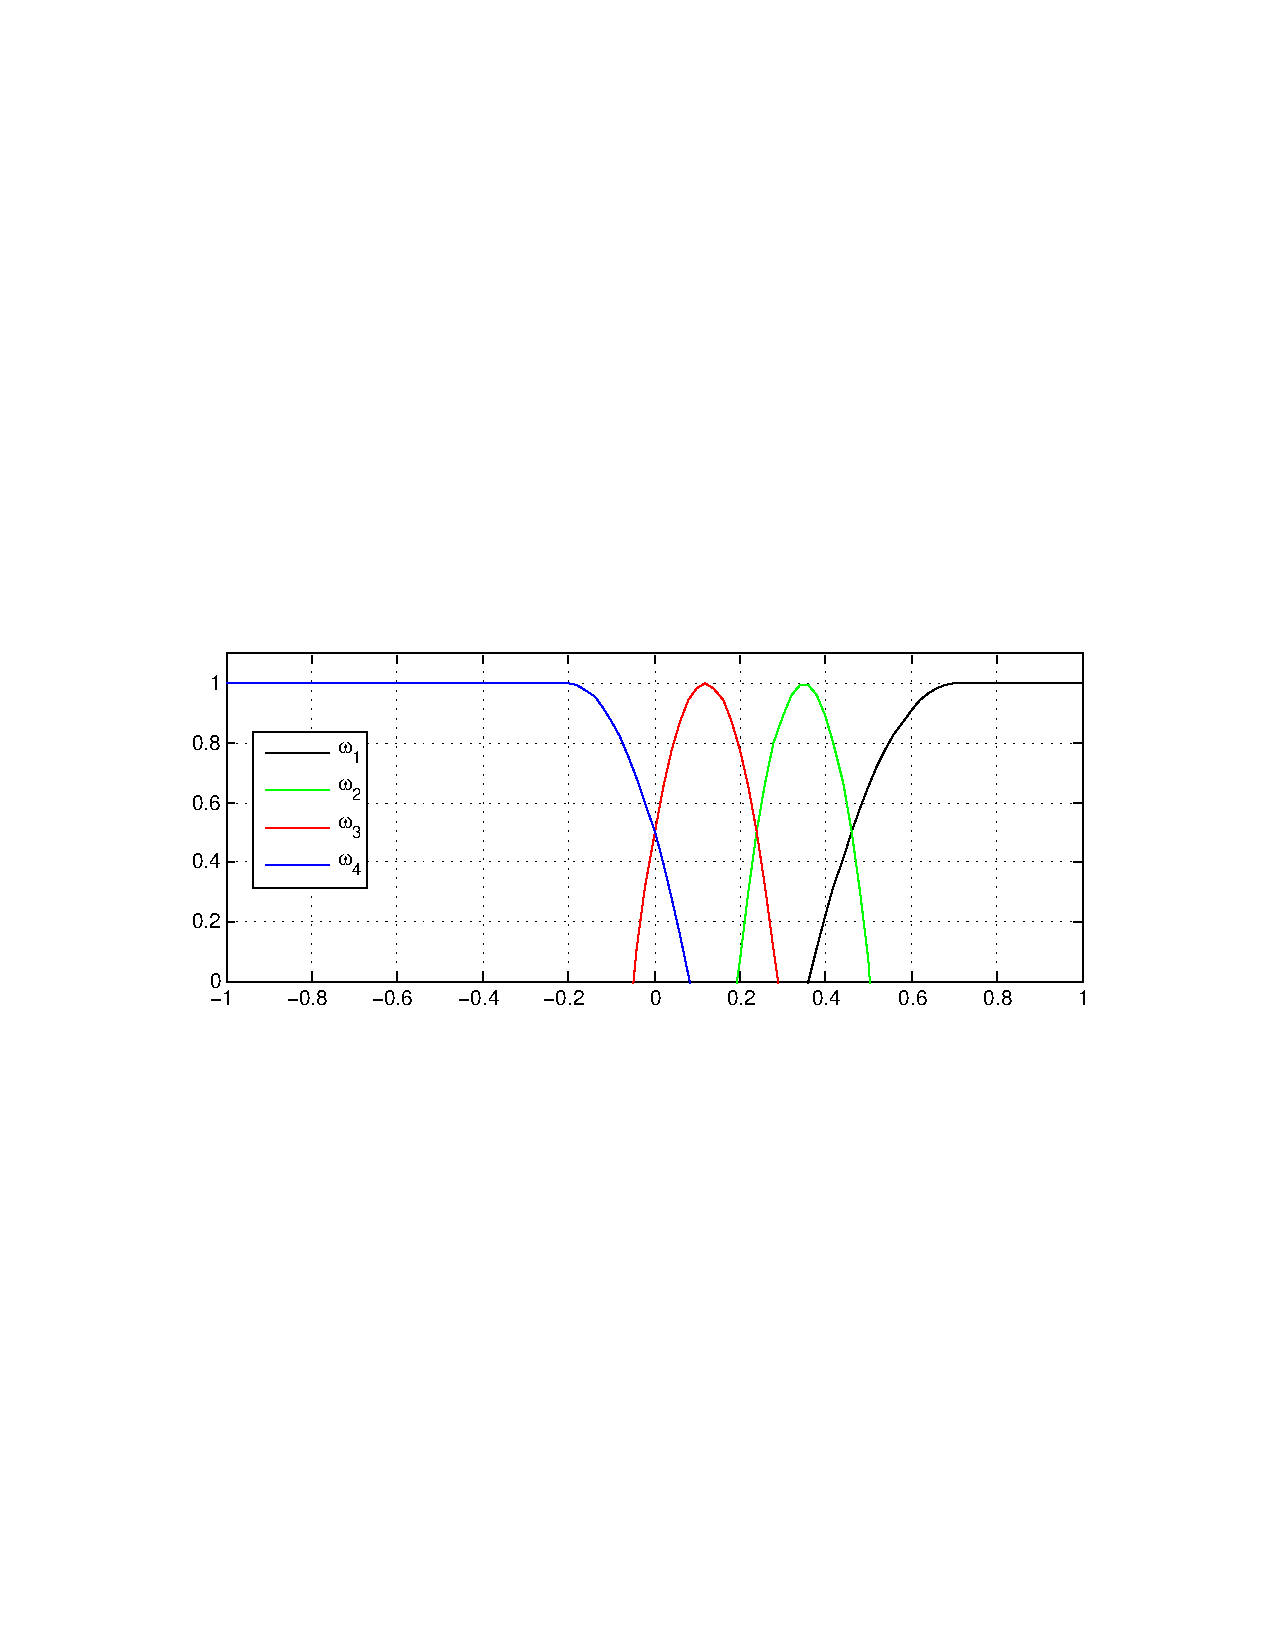
\includegraphics[trim = 30mm 108mm 30mm 110mm, clip,width=0.99\linewidth]{../images/parabola_omega.pdf}
      \caption{Parabolic functions $\Lambda_c,\, c=1,\ldots, 4$ for the four classes.}
       \label{fig:parabola}
   \end{figure}


%\begin{framebox}

\begin{table}[t]
		\centering
	\begin{subtable}[t]{0.21\textwidth}
		\centering
		\begin{tabular}{ | c| c | c | p{5cm} |} 
    		\hline
    		\; & cluster centers $m_c$  \\ \hline
    		$\omega_4$ & -0.2 \\  \hline
    		$\omega_3$ &  0.12  \\ \hline
    		$\omega_2$ &  0.35  \\ \hline
    		$\omega_1$ &   0.70\\
   		\hline
    \end{tabular}
    \caption{} 
    \label{table_cluster}
    \end{subtable}
%\end{center}
%\end{table}
%
%\begin{table}[t]
%\begin{center}
 	\begin{subtable}[t]{0.24\textwidth}
\centering
    		\vspace{-9mm}
   		\begin{tabular}{ | c| c | c | p{5cm} |} 
    		\hline
     		& transition values $b_k$\\ \hline
    		$\omega_4$/$\omega_3$ & 0  \\  \hline
    		$\omega_3$/$\omega_2$ &  0.24 \\ \hline
    		$\omega_2$/$\omega_1$ &  0.46  \\ \hline
    		 %&    \\ 
    		\end{tabular}
    		\vspace{3mm}
		\caption{} 
		\label{table_transition}
	\end{subtable}
			\caption{Class centers and transition values of the four detected classes.} 
\end{table}
%\end{framebox}

The row $P_{spec}(x_{i,j}|\omega_c)$ probabilities are used as initialization values for the membership probability $P(\omega_c | x_{i,j})$, which expresses the probability that the pixel $x_{i,j}$ is originated from a surface of type $\omega_c$.
The $P(\omega_c | x_{i,j})$ are then iteratively updated using the information from the neighborhood  $\Gamma (x_{i,j})$ of the pixel, which is constituted by the pixels contained in an $l\times l $  window centered in $x_{i,j}$, except $x_{i,j}$ itself. 
%The algorithm updates the membership weights of $P_{spec}(x|\omega_c)$ and considers contextual image informations.
%For this, the conditional spatial probability $P_{spat}(x_{i,j}|\omega _c)$ of each  $x_{(i,j)}$ must be computed.
%depends only on the pixels  $x'$ in its spatial neighborhood, $\Gamma (x)$. 
In order to take into account the interaction between neighboring pixels, Besag \cite{1986_besag} introduced the concept of  neighborhood potential $U(x_{i,j})$, which we compute as
%
\begin{equation} \label{U}
U(x_{i,j}|\omega_c) =   \sum_{x\in \Gamma (x_{i,j}) } [1-P(\omega_c|x)].
\end{equation}

Then, the spatial membership $P_{spat}(x_{i,j}|\omega_c)$ probability can be computed as:
%
\begin{equation} \label{spatial}
P_{spat}(x_{i,j}|\omega_c) = \gamma e^{-\beta U(x_{i,j}|\omega_c)}
\end{equation}
%
where $\beta$ is a positive coefficient used for weighting  the influence of the spatial context and $\gamma$ is a normalization factor such that $\sum_{c=1}^4 P_{spat}(x_{i,j}|\omega_c)=1$.
Anyway, it is not needed to actually compute $\gamma$ since it will elide in the next equation.
%
If $\beta$ is small the influence of the spatial contest will have an important weight in the final computation of $P_{spat}$.
%
%The value of $P_{spat}$ for the cluster $\omega_c$ if the neighboring pixels $x'$ have a big value of $P(\omega_c|x')$ for the same cluster $\omega_c$ and small if they belong to another class.
The last step is to compute the combined spectral-spatial probability $P(\omega_c|x_{i,j})$, which is also the total probability  assigned to a pixel $x_{i,j}$ to belong to a certain cluster $\omega_c$ 
%
\begin{eqnarray}  \label{spec_spat}
&&P(\omega_c|x_{i,j}) = \frac{P_{spec}(x_{i,j}|\omega_c) \cdot P_{spatial}(x_{i,j}|\omega_c) }{\sum_{c'}[P_{spec}(x_{i,j}|\omega_{c'}) \cdot P_{spatial}(x_{i,j}|\omega_{c'})]}  \nonumber\\
 &&\sum_{c=1}^n P(\omega_c|x_{i,j})=1
\end{eqnarray}

Equations  \eqref{U}-\eqref{spec_spat} are iteratively repeated for a fixed number of iterations (5 in our case), and the final $P(\omega_c|x_{i,j})$ can be used to create $Cl$ following a maximum probability criterion.

%We used an iteraive algorithm. To compute the following iterations, we only have updated the values of $P(\omega_c|x)$ with the values of $P_{spatial}(x|\omega_c)$ but without refresh the values of $P_{spec}(x|\omega_c)$.

%In this specific work, our task was to find four macro-areas,  $\omega_c$  $(c=1,2,3,4)$: water, soil, grass and trees. 
%In the table~\ref{table_cluster} , there are  the initial values chosen for the four center of the clusters, $m_c$. The transition values from one cluster to another, $b_{k}$ $(k=1,2,3)$ are in the table~\ref{table_transition}. To calculate $U$ the window size was $l=5$ and to estimate  $P_{spatial}$ in the  (\ref{spatial}) we used $\beta = 0.1$.


%To compute the probability of each pixel to belong to a cluster it is also possible to use a sigmoid  function. We got  very good results using both the functions.  But for running  online the software and getting real time results,  we decided to use  the parabola function, in fact  it takes less computational time and optimizes the process.









%%%%%%%%%%%%%%%%%%%%%%%%%%%%%%%%%%%%%%%%%%%%%%%%%%%%%%%%%%%%%%%%%%%%%%%%%%%%%%%%
\section{EXPERIMENTAL RESULTS}\label{sec:experimental_setup}


\begin{figure*}[t!]
      \centering
      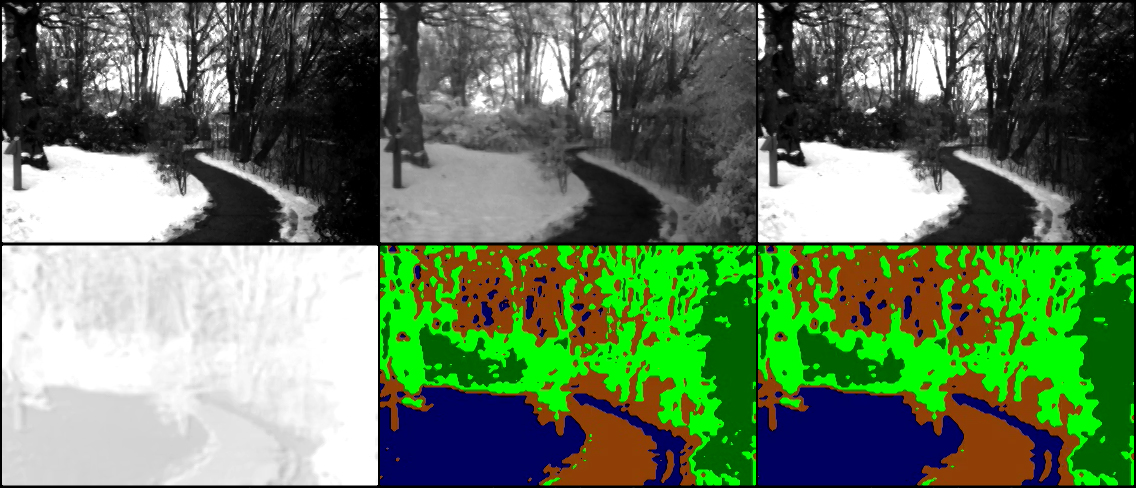
\includegraphics[width=0.99\textwidth]{../images/frame_1.jpg}
      \caption{Top: $RedL$, $NIRC$ and $RedR$ respectively; bottom: $NDVI$, the classification according to equation \eqref{ndvi_values} and the classified image after the clusterization.}
       \label{fig:frame1}
\end{figure*}




We have tested the developed system collecting multiple videos using a handheld version of the camera during multiple experimental sessions around the campus of the Max Planck Institute for biological Cybernetics, T{\"u}bingen, Germany.
All the computations to process the videos are performed online producing a classified image, disparity map and 3D point cloud at about 2Hz.




%During the experiments, we have handled  the camera and walked around recording and processing the video. In the  \ref {subsec:discussion} we are going  to discuss the frames taken by the filters/camera system (RedL, RedR and $NIRC$), the NDVI black and white frame and  the classification with and without clusterization.

%In this paper we are going to show the result got in a typical German winter day.  The scenario of the selected experiment shown: a path (soil), the snow all around the path, and some vegetation on the boards of the path. We have chosen  this type of scenario because it includes all the macro-areas that by reference  of literature value is possible to detect using the NDVI. It is also possible to detect more types of macro-areas (materials), in fact we are making our own data base, the preliminary results are in (\ref{fig:boxplot}).



%\subsection{Discussion}\label{subsec:discussion}

An example of the collected and classified images is shown in Fig. \ref{fig:frame1}.
On top, from left to right, we show the three camera inputs $RedL$, $NIRC$ and $RedR$.
The scene, includes a concrete path in the center, snow on the left, some vegetation on the right and in the background.
In $NIRC$, it is possible to observe the bright color of the vegetation, which means a high reflectance value in the NIR band.
Instead,  in the images acquired with the red filter $RedL$ and $RedR$ the vegetation appears darker.
Although the snow looks bright in both bandwidth, it is brighter in the red band.
Finally the concrete path shows a low reflectance in both bands.

The bottom raw shows in order the raw NDVI matrix $NDVI$, the image classified according to equation \eqref{ndvi_values} and the classified image after the clusterization.
In order to highlight the differences among the various classes, in the left image the NDVI values $-1 \leq NDVI \leq 1$ are scaled to the set $127 \leq  NDVI \leq 255$.
The snow, assuming negative NDVI values, is the darkest part, followed by the concrete, while the vegetation is relatively bright.
The central frame shows the classification of the image according to equation \eqref{ndvi_values}, where blue, brown, green and dark green areas represent respectively snow/water, soil/concrete, dry vegetation and healthy vegetation.
Although the classification performed in the central frame is already quite accurate, the right frame shows less noise and outliers.

A second example showing a closer point of view is provided in Fig. \ref{fig:frame2}, whose subject is a small tree about 70cm tall.
In addition to $RedL$, $NIRC$, $NDVI$ and the classified image, we show also the 3D reconstruction of the healthy vegetation present in the image, which includes the tree itself and some small areas on the left of the image.
This information, together with the classification, can be particularly useful to not only identify a landmark in the environment  and its bearing with respect to the camera frame, but also to produce  estimates of its distance and size.
The interested reader is invited to watch the videos collected during these experiments in the accompanying multimedia material.

%\paolo{decribe \ref{fig:boxplot}}
In order to verify that the data obtained by our sensor are consistent with the NDVI values found in literature, we have built a database of materials from our experiments.
In particular, for each material we have selected multiple points ($\geq 100$) over multiple frames of many different  experiments and computed the mean and covariance values of the corresponding NDVI values.
%We have done this check  selecting from different videos  frames with the presence of a specific material.  E.g. to check the mean NDVI value for the snow, we have taken five frames  from the initial video and selected one hundred points (pixels) with the snow, then we have taken the correspondent pixel in the  NDVI 1D matrix and saved the pixel value.  Once collected all the one hundred value we have made a statistical analysis ().
Fig. \ref{fig:boxplot} shows the results of this statistical analysis. 
The median for each material is shown as a red horizontal line, while $50\%$ of the collected data fits in the blue boxes, known as the inter-quartile range (IQR).
The extreme values (within 1.5 times the inter-quartile range from the upper or lower quartile) are the ends of the dashed vertical lines extending from the IQRs.
Points at a greater distance from the median than 1.5 times the IQR are plotted individually as red pluses and are considered potential outliers.

We have studied classes of material as water, asphalt, snow, concrete, plant stems and leaves. 
The results obtained are all congruent with the values obtained from literature, with the notable exception of asphalt, for which we expected a  slightly greater value.
Nevertheless, this discrepancy may be due  either to a not perfect tuning of the cameras or to the particular observed asphalt.
Nevertheless, the computed values can be used in future to build a more refined classification with more classes.


\begin{figure*}[t!]
      \centering
      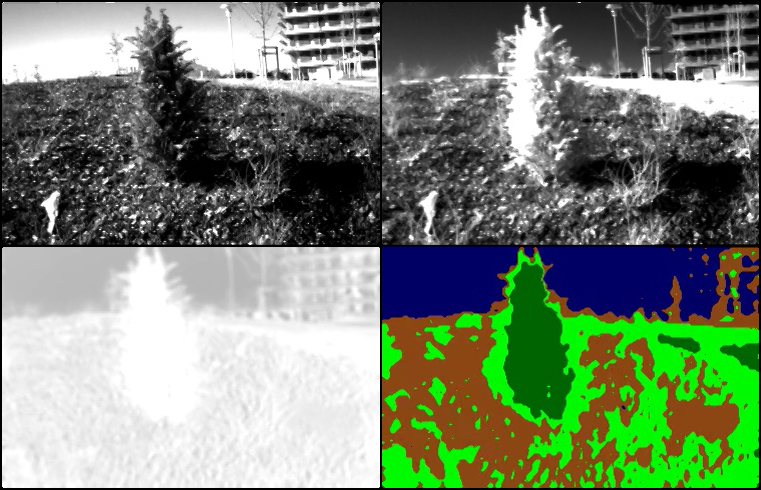
\includegraphics[width=0.57\textwidth]{../images/frame_2.jpg}
      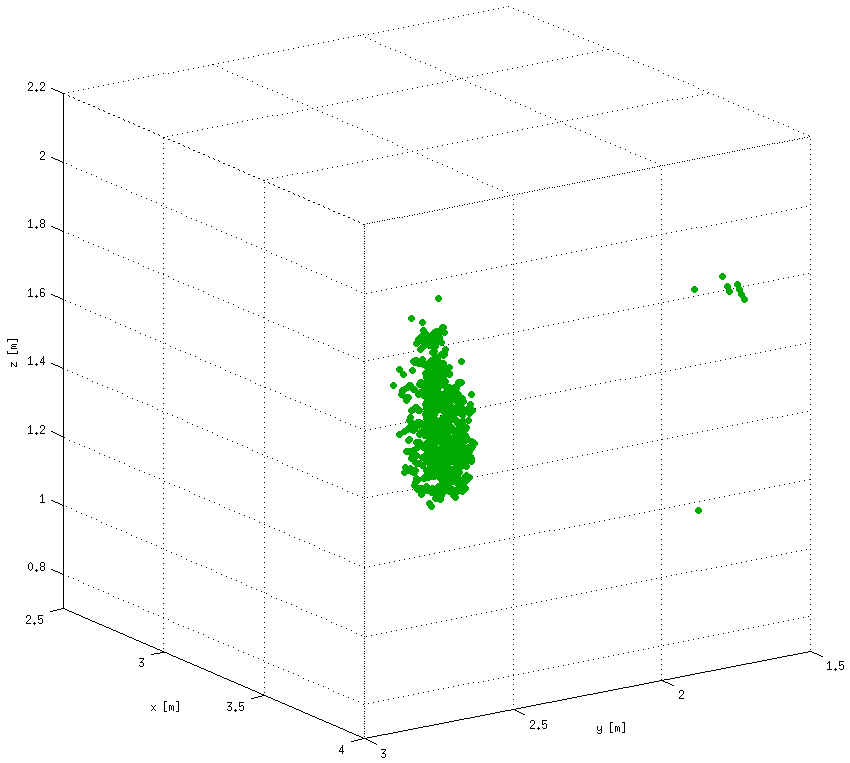
\includegraphics[width=0.41\textwidth]{../images/frame_2pc.jpg}
      \caption{Top-left: $RedL$ and $NIRC$ respectively; bottom-left: $NDVI$, the classification and the classified image after the clusterization; right: the reconstructed point-cloud of the healthy vegetation class only.}
       \label{fig:frame2}
\end{figure*}



\begin{figure}[t]
      \centering
      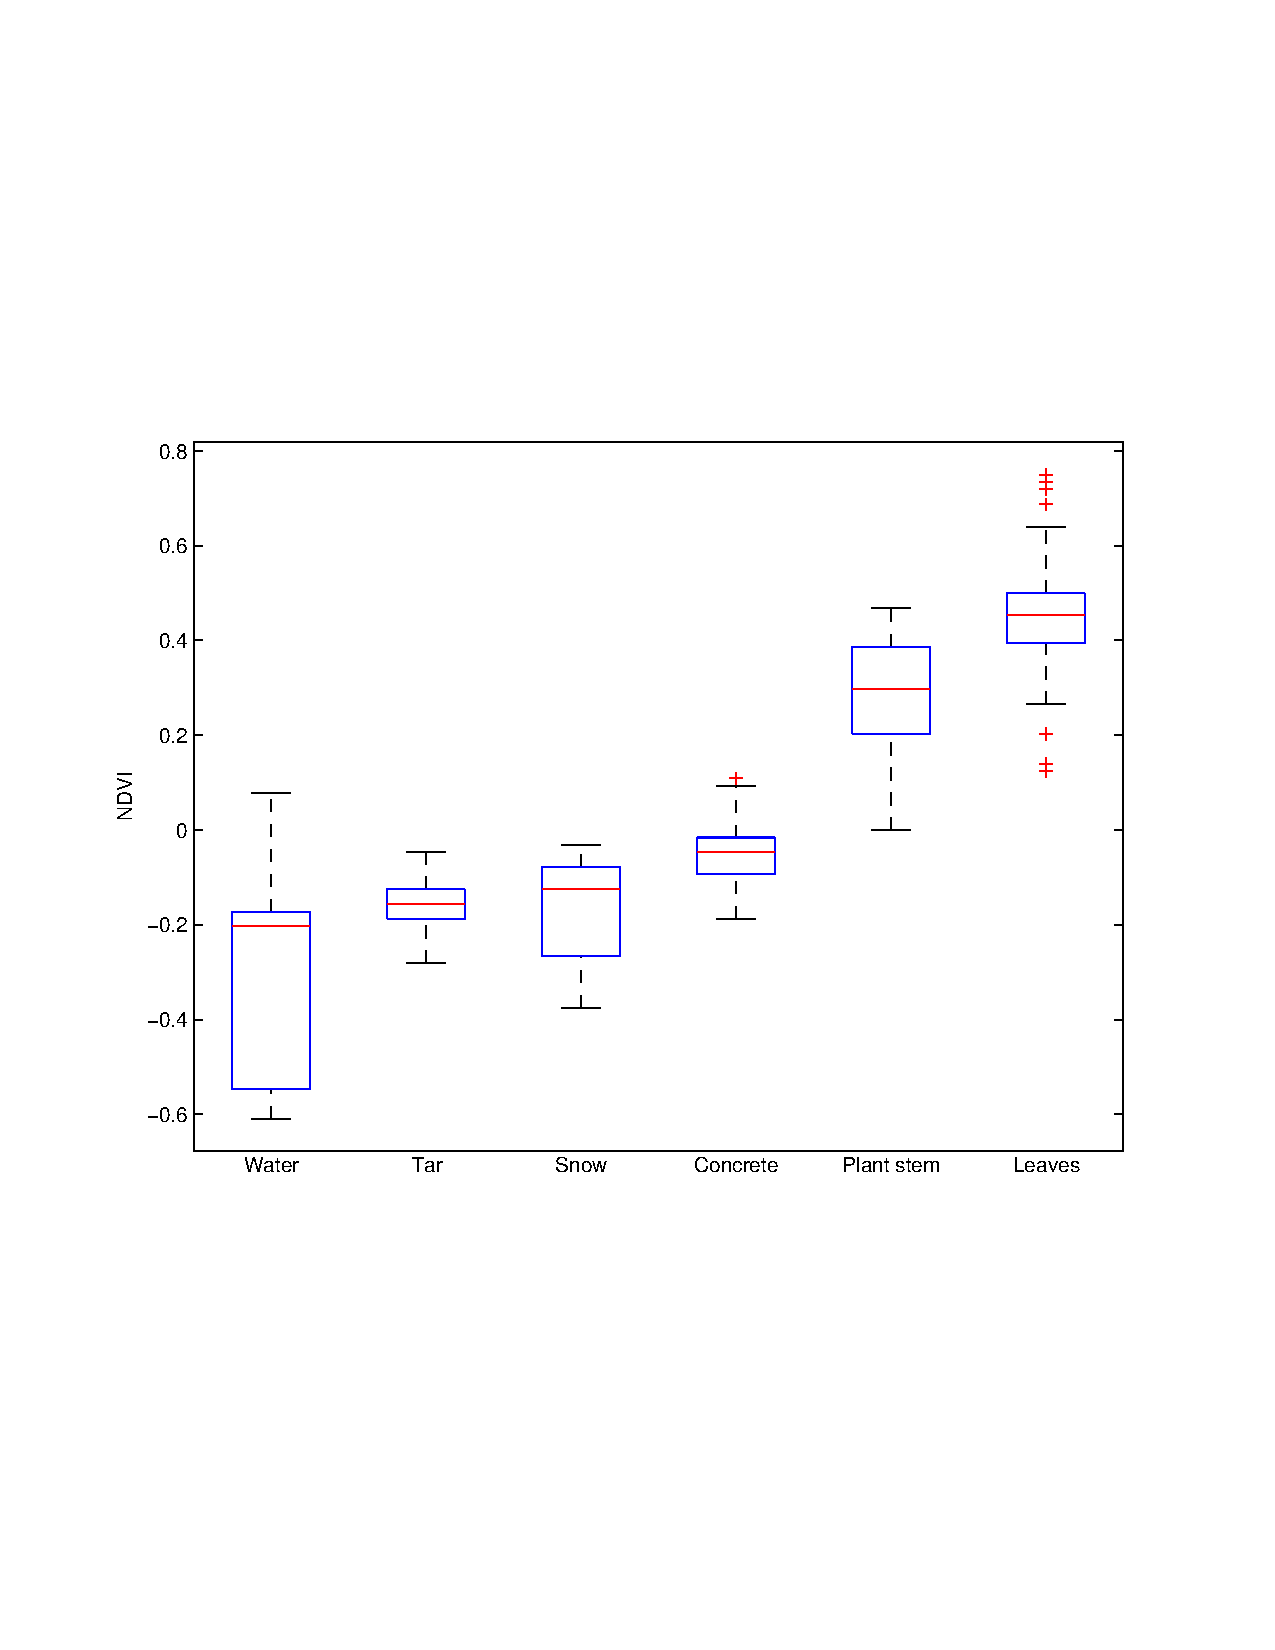
\includegraphics[trim = 1mm 75mm 1mm 75mm, clip,width=0.99\linewidth]{../images/experiment/boxplot_database.pdf}
      \caption{Quartiles of the NDVI values taken by the camera sensor for six different materials: water, asphalt, snow, concrete, plant steam and leaves}
       \label{fig:boxplot}
   \end{figure}

 

%%%%%%%%%%%%%%%%%%%%%%%%%%%%%%%%%%%%%%%%%%%%%%%%%%%%%%%%%%%%%%%%%%%%%%%%%%%%%%%%
\section{CONCLUSIONS}\label{sec:conclusions}

In this work, we have designed and implemented a low-cost low-weight sensor that is able to work both as spectral and stereo camera, consisting of a camera array with appropriate filters.
The combination of these two sensors allows the extraction of information on the material of the observed objects and on their distance.
As ultimate result, we are able to create a pointcloud of some selected features, as for example trees,  that can be efficiently used, among other applications, as landmarks in outdoor navigation.

In future, we plan to optimize our software and port it to a more compact platform as Odroid XU which can be embedded on a UAV, having as final goal the processing of the information at $10Hz$.
As for further development of the classification itself, we plan to test the sensor with multiple materials to create our own database and refine the number and parameters of the classes.
In addition we would like to study how to exploit the depth-map also during the fuzzy classification.
Finally, we plan to apply the extracted information to outdoor navigation for landmark-based navigation and identification of safe landing areas.



%%%%%%%%%%%%%%%%%%%%%%%%%%%%%%%%%%%%%%%%%%%%%%%%%%%%%%%%%%%%%%%%%%%%%%%%%%%%%%%%
\bibliographystyle{IEEEtran}
\bibliography{IEEEabrv,mybibfile}














%%%%%%%%%%%%%%%%%%%%%%%%%%%%%%%%%%%%%%%%%%%%%%%%%%%%%%%%%%%%%%%%%%%%%%%%%%%%%%%%



%%%%%%%%%%%%%%%%%%%%%%%%%%%%%%%%%%%%%%%%%%%%%%%%%%%%%%%%%%%%%%%%%%%%%%%%%%%%%%%%








   



%%%%%%%%%%%%%%%%%%%%%%%%%%%%%%%%%%%%%%%%%%%%%%%%%%%%%%%%%%%%%%%%%%%%%%%%%%%%%%%%



%%%%%%%%%%%%%%%%%%%%%%%%%%%%%%%%%%%%%%%%%%%%%%%%%%%%%%%%%%%%%%%%%%%%%%%%%%%%%%%%



%%%%%%%%%%%%%%%%%%%%%%%%%%%%%%%%%%%%%%%%%%%%%%%%%%%%%%%%%%%%%%%%%%%%%%%%%%%%%%%%




%%%%%%%%%%%%%%%%%%%%%%%%%%%%%%%%%%%%%%%%%%%%%%%%%%%%%%%%%%%%%%%%%%%%%%%%%%%%%%%%








\end{document}